\section{Desigualdade de Clausius}

A Desigualdade de Clausius é um corolário da Segunda Lei, para qualquer ciclo e qualquer corpo ou conjunto de corpos pelos quais o ciclo troca energia por calor. Este corolário é uma base para o entendimento da entropia.

\begin{equation}
    \oint \left( \frac{\delta Q}{T} \right)_b \leq 0 
\end{equation}

onde $\delta Q$ representa o calor transmitido numa parte da fronteira do sistema, a uma temperatura $T$. A integração é feita ao longo de toda a fronteira (``b'' de \textit{boundary}) e durante um ciclo completo. $\int_t \int_A \left( \frac{\delta q (x,y,z,t)}{T(x,y,z,t)} \right)_b \leq 0$.
Tal como em Kelvin-Planck \autoref{thm:kelvin-planck}, a igualdade aplica-se quando não há irreversibilidades internas, e a desigualdade quando as há.

\begin{proof}
    Um sistema recebe $\delta Q$ numa parte da sua fronteira à temperatura $T$, desenvolvendo $\delta W$. $\delta Q$ é recebido de um reservatório a $T_{res}$. Para evitar a existência de irreversibilidades no sistema, devido à diferença de temperatura entre o reservatório e o sistema, um sistema intermédio que opera num ciclo reversível pode ser colocado entre estes. Este recebe $\delta Q'$ do reservatório e cede $\delta Q$ ao sistema, enquanto produz $\delta W'$.
    Como visto anteriormente, podemos escrever:
    \begin{equation*}
        \left( \frac{\delta Q'}{\delta Q} \right)_{rev} = \frac{T_{res}}{T} \Longleftrightarrow \frac{\delta Q'}{T_{res}} = \left( \frac{\delta Q}{T} \right)_b
    \end{equation*}
    Se a temperatura $T$ variar, uma multiplicidade de ciclos reversíveis intermédios poderão ser necessários.
    Considerando, agora, o balanço energético do sistema constituído pelos dois sistemas, o intermédio e o inicial, sem assumir direções de transferência:
    \begin{equation*}
        d E_T = \delta Q' + \delta W_T \Longleftrightarrow \delta W_T = - T_{res} \left( \frac{\delta Q}{T} \right)_b + d E_T
    \end{equation*}
    O sistema conjunto opera num ciclo, pois as suas partes operam num ciclo. Deixando o sistema executar um ciclo completo (o ciclo intermédio pode realizar mais do que um), o trabalho total do sistema conjunto é:
    \begin{equation*}
        \oint \delta W_T = - \oint T_{res} \left( \frac{\delta Q}{T} \right)_b + \cancelto{0}{\oint d E_T} = - T_{res} \oint \left( \frac{\delta Q}{T} \right)_b
    \end{equation*}
    $T_{res}$ é constante, pela definição de reservatório, pelo que pode sair para fora do integral, e a variação de energia no ciclo é zero por definição.
    O sistema conjunto comunica com apenas um reservatório, pelo que, de Kelvin-Planck \autoref{thm:kelvin-planck}, $\oint \delta W_T \geq 0$. Como $- T_{res} < 0$, temos obrigatoriamente que $\oint \left( \frac{\delta Q}{T} \right)_b \leq 0$.
    
    Sabemos também de Kelvin-Planck que a igualdade aplica-se quando não há irreversibilidades internas no sistema inicial, e a desigualdade quando as há, dado que o sistema intermédio é reversível.
\end{proof}


Definindo

\begin{equation}
    \sigma \equiv - \oint \left( \frac{\delta Q}{T} \right)_b \quad
    \begin{cases}
        0, & \text{reversível (ideal)} \\
        > 0, & \text{irreversível (real)}
    \end{cases}
\end{equation}

O termo $\sigma$ pode ser interpretado como a entropia gerada durante um ciclo devido às irreversibilidades internas. $\sigma$ não pode ser negativo.  


\section{Definição Entropia}

Um sistema fechado executa dois ciclos. Sejam $A$, $B$ e $C$ processos internamente reversíveis, o primeiro ciclo consiste do processo A do estado 1 para o estado 2, seguido do processo C do estado 2 para o estado 1. O segundo ciclo consiste do processo B do estado 1 para o estado 2, seguido do processo C do estado 2 para o estado 1.

Da Desigualdade de Clausius,

\begin{equation*}
    \oint \left( \frac{\delta Q}{T} \right)_{AC}  = \left( \int_1^2 \frac{\delta Q}{T} \right)_A + \left( \int_2^1 \frac{\delta Q}{T} \right)_C = - \cancelto{0}{\sigma_{AC}}
\end{equation*}

\begin{equation*}
    \oint \left( \frac{\delta Q}{T} \right)_{BC}  = \left( \int_1^2 \frac{\delta Q}{T} \right)_B + \left( \int_2^1 \frac{\delta Q}{T} \right)_C = - \cancelto{0}{\sigma_{BC}}
\end{equation*}

Os termos de geração de entropia $\sigma_{ciclo} = 0$, pois os ciclos são compostos por processos internamente reversíveis.

Deste modo,

\begin{equation*}
    \left( \int_1^2 \frac{\delta Q}{T} \right)_A = \left( \int_1^2 \frac{\delta Q}{T} \right)_B
\end{equation*}

Como $A$ e $B$ são arbitrários, segue que o integral de $\frac{\delta Q}{T}$ tem o mesmo valor para quaisquer dois processos internamente reversíveis entre os mesmos dois estados. Desta forma, o valor do integral é independente do processo, e só depende dos estados inicial e final.

Por isso, o integral representa a variação de uma propriedade do sistema.

Definindo $S$ para entropia:

\begin{equation} \label{eq:def-entropia-rev}
    S_2 - S_1 = \left( \int_1^2 \frac{\delta Q}{T} \right)_{rev} \quad \text{ou, na forma diferencial:} \quad dS = \left( \frac{\delta Q}{T} \right)_{rev}
\end{equation}

onde $S$ é uma propriedade extensiva. As unidades SI são J/K.

É importante reforçar que a variação de entropia depende apenas dos estado inicial e final, não importando se ocorreu um processo reversível ou irreversível.

Quando um sistema fechado sob um processo internamente reversível, recebe energia por calor, a entropia do sistema aumenta, e vice-versa. A transferência de entropia acompanha a transferência de calor.

\section{Balanço de Entropia para Sistemas Fechados}

Considerando, agora, um sistema fechado que opera num ciclo, sendo $A$ um processo irreversível do estado 1 para o estado 2, e $B$ um processo reversível de 2 para 1. Tem-se

\begin{equation*}
    \left( \oint \frac{\delta Q}{T} \right)_{AB} = \left( \int_1^2 \frac{\delta Q}{T} \right)_A + \left( \int_2^1 \frac{\delta Q}{T} \right)_B =  - \sigma_{AB} 
\end{equation*}

Como $B$ é reversível, $S_1 - S_2 = \left( \int_2^1 \frac{\delta Q}{T} \right)_B$. Logo, o balanço de entropia de um sistema fechado é:

\begin{equation}
    S_2 - S_1 = \int_1^2 \left( \frac{\delta Q}{T} \right)_b + \sigma_{12} \quad \text{ou, na forma diferencial:} \quad dS = \left( \frac{\delta Q}{T}  \right)_b + d\sigma
\end{equation}

O balanço de entropia diz-nos por palavras que a variação de entropia de um sistema num dado intervalo de tempo é igual ao resultado de transferência de entropia pela fronteira nesse intervalo de tempo, somado à entropia gerada dentro do sistema nesse intervalo de tempo.
A entropia é gerada dentro do sistema devido às irreversibilidades internas, que depende do processo e não apenas dos estados inicial e final, pelo que a geração de entropia, $\sigma$, não é uma propriedade.

Num sistema, comparando a geração de entropia de cada componente de um sistema, consegue-se diminuir as ineficiências do sistema. O termo de transferência de entropia requer informação da transferência de calor e da temperatura na fronteira, o que pode não ser conveniente. Pode-se alargar a fronteira do sistema, de forma a que a temperatura na fronteira seja aproximadamente constante. No entanto, seria necessário contar com os efeitos de geração de entropia causados pela porção da vizinhança incluída. 


\section{Tabelas \& Entropia}

Os valores de entropia específica são dados relativamente a uma dada referência. Para a água líquida saturada a $0.01 \text{\textdegree C}$ a entropia é definida a zero. Para os refrigerantes, é definida a zero para o estado líquido saturado a $-40 \text{\textdegree C}$.

\begin{equation}
    S = S_0 + \left( \int \frac{\delta Q}{T} \right)_{rev}
\end{equation}

\begin{equation*}
    s = (1-x) s_f + x s_g = s_f + x (s_g - s_f)
\end{equation*}

Não havendo dados de líquido comprimido, o valor da entropia específica pode ser estimado, tal como para $v$ e $u$, usando o valor do líquido saturado à mesma temperatura: $s(T,p) \approx s_f(T)$.


\section{Geração de Entropia}

\subsection{Gradiente de Pressão}

Considerando um sistema êmbolo-cilindro adiabático a ser comprimido, temos \newline $du = \cancelto{0}{\delta Q} + \delta W \implies du = - p_{ext} dv$. Por outro lado, usando a Equação \ref{eq:1tds}, sabendo que o sistema dentro do cilindro está sob a pressão $p_{int}$: $du = T ds - p_{int} dv$ e, sendo adiabático, $ds = \cancelto{0}{\frac{\delta Q}{T}} + \delta \sigma$. Temos, então:

\begin{equation*}
    -p_{ext} dv = T \delta \sigma - p_{int} dv \implies \delta \sigma = \frac{(p_{int} - p_{ext}) dv}{T}
\end{equation*}

Assim, para um processo lento, temos que em cada momento $p_{int} \approx p_{ext}$, pois é dado tempo suficiente para que a pressão transmitida ao êmbolo se uniformize dentro do cilindro. Desta forma, $\delta \sigma \approx 0$, i.e. um processo lento aproxima-se de um processo ideal reversível, onde não se gera entropia.

Por outro lado, para um processo rápido, num instante de tempo após ser aplicado a força, a $p_{ext}$ será superior à $p_{int}$. Esta diferença será tanto maior quando mais rápido o processo, pois dá-se menos tempo ao sistema para este atingir o equilíbrio mecânico. Assim, $p_{int} \neq p_{ext}$ e $p_{int} < p_{ext}$, pelo que $(p_{int} - p_{ext})dv > 0$ e, quanto mais rápido o processo, maior a diferença instantânea de pressão, $(p_{int} - p_{ext})dv \uparrow \implies \delta \sigma \uparrow$. Deste modo, quanto mais rápido o processo e maior o gradiente de pressão, maior é a geração de entropia. Descobrimos, então, que $\sigma \propto \nabla p$.

Além disso, de $-p_{ext} dv = T ds - p_{int} dv$, induzimos que, nos ciclos, é necessário libertar energia na forma de calor, de forma a diminuir a temperatura ($Tds \downarrow$), de tal forma a que $p_{int} \approx p_{ext}$.

\subsection{Gradiente de Temperatura}

Considerando um sistema isolado e rígido, constituído por dois subsistemas $A$ e $B$, existe uma parede rígida entre ambos que inicialmente é adiabática e depois deixa de ser.

O balanço de entropia para o sistema todo dá: $dS = \cancelto{0}{\frac{\delta Q}{T}} + \delta \sigma \Longleftrightarrow dS_A + dS_B = \delta \sigma \Longleftrightarrow \frac{\delta Q_A}{T_A} + \cancelto{0}{\delta \sigma_A} + \frac{\delta Q_B}{T_B} + \cancelto{0}{\delta \sigma_B} = \delta \sigma$.

O balanço energético de todo o sistema dá: $dU = \cancelto{0}{\delta Q} + \cancelto{0}{\delta W} \implies dU_A + dU_B = 0 \Longleftrightarrow \delta Q_A + \cancelto{0}{\delta W_A} + \delta Q_B + \cancelto{0}{\delta W_B} = 0 \implies \delta Q_A + \delta Q_B = 0$.

Como $Q_A = -Q_B$, concluimos que

\begin{equation*}
    \delta \sigma = \delta Q_B \left( \frac{1}{T_B} - \frac{1}{T_A} \right) = \delta Q_B \left( \frac{T_A - T_B}{T_A T_B} \right)
\end{equation*}

Assim, geração de entropia também está relacionada com a existência de diferenças de temperatura: $\sigma \propto \delta Q \frac{\nabla T}{T^2}$.

A geração de entropia também está relacionada com a viscosidade do fluido.


\section{Equações TdS}

Num sistema compressível sob um processo internamente reversível (ignorando energia cinética e potencial do sistema), temos $dU = \delta Q + \delta W$. Sendo internamente reversível podemos usar a equação \ref{eq:def-entropia-rev} ($dS = \frac{\delta Q}{T}$) e $\delta W = -p dV$:

\begin{equation} \label{eq:1tds}
    T dS = dU + p dV
\end{equation}

Esta é a 1ªEquação $TdS$.

Seja $u = \mathbf{u}[p, v]$, tem-se $du = \frac{\partial u}{\partial s}\bigr|_{v} ds + \frac{\partial u}{\partial v}\bigr|_{s} dv \Longleftrightarrow du = T ds - p dv$, pelo que 

\begin{eqnarray}
    T = \frac{\partial u}{\partial s}\bigr|_{v} \qquad T = \frac{\partial U}{\partial s}\bigr|_{M,v}\\
    p = - \frac{\partial u}{\partial v}\bigr|_{s} \qquad p = - \frac{\partial U}{\partial v}\bigr|_{M,s}
\end{eqnarray}


Sabendo que $h = u + pv \implies dh = du + pdv + vdp \Longleftrightarrow du+pdv = dh - vdp$. Substituindo na Equação \ref{eq:1tds}, chegamos à 2ªEquação $TdS$:

\begin{equation} \label{eq:2tds}
    Tds = dh - v dp \quad \text{ou} \quad TdS = dH - Vdp
\end{equation}

Embora estas equações foram derivadas considerando processos reversíveis, a diferença de entropia obtida integrando estas equações é a variação de entropia entre dois estados de equilíbrio, independentemente do processo ser reversível ou irreversível, pois a entropia é uma propriedade.

Considerando um mudança de fase de líquido saturado para vapor saturado a pressão e temperatura constante, por \ref{eq:2tds}, $ds = \frac{dh}{T}$, obtemos uma fórmula para calcular $s_g - s_f = \frac{h_g - h_f}{T}$.

\section{Variação de Entropia para Substâncias Incompressíveis}

O modelo de uma substância incompressível assume que $dv = 0$ e, portanto, $du = c(T) dT$. Usando a Equação \ref{eq:1tds}, 

\begin{equation*}
    ds = \frac{du}{T} + \frac{p dv}{T} = \frac{c(T) dT}{T}
\end{equation*}

Pelo que

\begin{equation*}
    s_2 - s_1 = \int_{T_1}^{T_2} \frac{c(T) dT}{T}
\end{equation*}

Quando o calor específico é constante, temos

\begin{equation*}
    s_2 - s_1 = c \ln \frac{T_2}{T_1}
\end{equation*}

Uma aplicação desta equação está presente no Exemplo \ref{ex:Temperatura Final}.

\section{Variação de Entropia para Gás Ideal}

Reescrevendo a Equação \ref{eq:1tds} como: $ds = \frac{du}{T} + \frac{p}{T} dv$, e a Equação \ref{eq:2tds} como: $ds = \frac{dh}{T} - \frac{v}{T} dp$

Para um gás ideal: $du = c_v dT$, $dh = c_p dT$ e $pv = RT$: $ds = c_v \frac{dT}{T} + R\frac{dv}{v}$ e $ds = c_p \frac{dT}{T} - R\frac{dp}{p}$.

Integrando:

\begin{equation} \label{eq:gas-int}
    s_2 - s_1 = \int_{T_1}^{T_2} c_v (T) \frac{dT}{T} + R \ln \frac{v_2}{v_1} \quad \text{e} \quad s_2 - s_1 = \int_{T_1}^{T_2} c_p (T) \frac{dT}{T} - R \ln \frac{p_2}{p_1}
\end{equation}

Assumindo $c_p$ e $c_v$ constantes,

\begin{equation}
    s_2 - s_1 = c_v \ln \frac{T_2}{T_1} + R \ln \frac{v_2}{v_1} \quad \text{e} \quad s_2 - s_1 = c_p \ln \frac{T_2}{T_1} - R \ln \frac{p_2}{p_1}
\end{equation}

Usando $pv = RT$ na primeira equação temos:

\begin{equation*}
    s_2 - s_1 = c_v \ln \frac{p_2 v_2}{p_1 v_1} + R \ln \frac{v_2}{v_1} = c_v \ln \frac{p_2}{p_1} + c_v \ln \frac{v_2}{v_1} + R \ln \frac{v_2}{v_1}
\end{equation*}

Como $c_p = c_v + R$, obtemos a última equação:

\begin{equation} \label{eq:cpcv}
    s_2 - s_1 = c_v \ln \frac{p_2}{p_1} + c_p \ln \frac{v_2}{v_1} 
\end{equation}

\subsection{Consulta de Tabelas para Gás Ideal}

Para um gás ideal, não considerando $c_p$ e $c_v$ constantes, os valores de entropia estão tabelados. Defina-se para uma temperatura arbitrária $T'$:

\begin{equation}
    s^0(T) = \int_{T'}^T \frac{c_p(T)}{T} dT
\end{equation}

Como,

\begin{equation*}
    \int_{T_1}^{T_2} c_p \frac{dT}{T} = \int_{T'}^{T_2} c_p \frac{dT}{T} - \int_{T'}^{T_1} c_p \frac{dT}{T} = s^0(T_2) - s^0(T_1)
\end{equation*}

Então, a Equação \ref{eq:gas-int} pode ser reescrita como:

\begin{equation} \label{eq:s0}
    s_2 - s_1 = s^0(T_2) - s^0(T_1) - R \ln \frac{p_2}{p_1}
\end{equation}

Como $s^0$ depende apenas da temperatura, pode ser tabulado em função da temperatura, tal como $h$ e $u$. Para o ar, como gás ideal, $s^0$ é dado na tabela Tab. A-22, e na Tab. A-23 para outros gases.

\section{Processo Isentrópico para Gás Ideal}

Para um processo isentrópico de um gás ideal, temos da equação \ref{eq:s0}: 

\begin{equation} \label{eq:tab1}
    s^0(T_2) = s^0(T_1) + R \ln \frac{p_2}{p_1}
\end{equation}

onde podemos obter $T_2$ sabendo $T_1$ e consultando na tabela os valores das entropias específicas $s^0(T_1)$ e $s^0(T_2)$.

\subsection{Ar}

Para o Ar, existe outra possibilidade de consulta para um processo \textbf{isentrópico}, na Tab. A-22. A partir da equação \ref{eq:tab1}:

\begin{eqnarray}
    \frac{s^0(T_2) - s^0(T_1)}{R} = \ln \frac{p_2}{p_1} \nonumber \\
    p_2 = p_1 \exp \left[\frac{s^0(T_2) - s^0(T_1)}{R} \right] \nonumber \\
    p_2 = p_1 \frac{\exp(s^0(T_2)/R)}{\exp(s^0(T_1)/R)}
\end{eqnarray}

Como $\exp(s^0(T)/R)$ apenas depende da temperatura, pode-se escrever $p_r(T) = \exp(s^0(T)/R)$ e, então:

\begin{equation} \label{eq:pr}
    \frac{p_2}{p_1} = \frac{p_{r2}}{p_{r1}} 
\end{equation}

Os valores tabelados para a pressão relativa $p_r$ são divididos por um fator, porque esta definição daria valores muito elevados.

Usando a equação de estado do modelo de gás ideal obtemos ainda o volume relativo $v_r$:

\begin{eqnarray}
    \frac{v_2}{v_1} = \frac{RT_2}{p_2} \frac{p_1}{RT_1} \nonumber  \\
    \frac{v_2}{v_1} = \frac{RT_2}{p_{r2}} \frac{p_{r1}}{RT_1} \nonumber \\
    \frac{v_2}{v_1} = \frac{v_{r2}}{v_{r1}}  \label{eq:vr}
\end{eqnarray}

Reforço que estas duas fórmulas (\ref{eq:pr} e \ref{eq:vr}) só se verificam para \textbf{processos isentrópicos} para o \textbf{Ar}.

\subsection{Processo Politrópico n=k}

Por outro lado, da equação \ref{eq:cpcv}:

\begin{equation}
    \cancelto{0}{\Delta s} = c_v \ln \frac{p_2}{p_1} + c_p \ln \frac{v_2}{v_1} \Longleftrightarrow \ln \frac{p_2}{p_1} + \frac{c_p}{c_v} \ln \frac{v_2}{v_1} = 0 \Longleftrightarrow \ln \left[ \frac{p_2}{p_1} \left( \frac{v_2}{v_1} \right)^{\frac{c_p}{c_v}} \right] = 0
\end{equation}

\begin{equation}
    \frac{p_2}{p_1} = \left( \frac{v_1}{v_2} \right)^{\frac{c_p}{c_v}}
\end{equation}

Assim, um processo isentrópico de um gás ideal é um processo politrópico ($pv^n = \text{const.}$) com: $n = \frac{c_p}{c_v} = k$.

Alternativamente, aplicando a equação dos gases ideais:

\begin{equation}
    \frac{T_2}{T_1} = \left( \frac{p_2}{p_1} \right)^{(k-1)/k} = \left( \frac{v_1}{v_2} \right)^{k-1}
\end{equation}

Segundo $ds = \frac{\delta Q}{T} + \delta \sigma$, se um processo é reversível e ocorre num sistema adiabático, o processo é isentrópico ($ds = \cancelto{0}{\frac{\delta Q}{T}} + \cancelto{0}{\delta \sigma}$). No entanto, o processo também pode ser isentrópico $\Delta S = 0$, se $\int \left( \frac{\delta Q}{T} \right)_b = - \sigma$, e, para isso, o sistema tem de ser arrefecido.

\textbf{NB:} Qualquer combinação de duas características das três: \{adiabático, reversível, isentrópico\}, implica a terceira.





\section{Entropia na Termodinâmica Estatística}

Num sistema isolado, considerando gás ideal, onde ocorre uma expansão $V_2 = 2 V_1$. A variação de entropia num processo a temperatura constante:

\begin{equation*}
    s_2 - s_1 = R \ln \left(\frac{v_2}{v_1}\right) \Longleftrightarrow S_2 - S_1 = m R \ln \left(\frac{v_2}{v_1}\right)  \Longleftrightarrow S_2 - S_1 = n \mathcal{R} \ln \left(\frac{v_2}{v_1}\right) 
\end{equation*}

Na termodinâmica estatística, os \textit{microestados} correspondem às diferentes combinações de posições e velocidades em que uma molécula pode estar. O número total de microestados é denominado ``probabilidade'' termodinâmica, $W=\frac{N!}{\prod_i N_i!}$, onde $N$ partículas idênticas das quais $N_i$ estão no microestado $i$. O numerador é uma correção, já que partículas idênticas no mesmo estado são indistinguíveis.

Se dois sisteamas são independentes, o número total de microestados é $W = W_A \cdot W_B$. Sendo uma propriedade extensiva, a entropia total de dois sistemas independentes é igual a soma de ambos $S(W) = S(W_A \cdot W_B) = S(W_A) + S(W_B)$. Ora, a função que satisfaz esta propriedade é o logarítmo.

Assim, para um sistema de $N$ partículas, a probabilidade termodinâmica é $w^N$, e a entropia é considerada proporcional a $\ln(w)^N$, ou $S \propto N \ln w$. A relação de Boltzmann é $S = N k_B \ln w$. Usando esta relação para calcular a variação de entropia temos: $S_2 - S_1 = N k_B \ln w_2 - N k_B \ln w_1 \Longleftrightarrow S_2 - S_1 = N k_B \ln \frac{w_2}{w_1}$. Ou seja, esta relação é válida para $k_B = \frac{n \mathcal{R}}{N} = \frac{\mathcal{R}}{N_A}$, onde $N_A$ é o número de Avogadro. e $\frac{v_2}{v_1} = \frac{w_2}{w_1}$. No nosso exemplo, $\frac{w_2}{w_1} = 2$, ou seja, ao duplicar o volume duplicou-se o número de microestados.

Deste modo, num sistema isolado, um processo, que aumente o número possível de microestados de um sistema, aumenta a sua entropia e vice-versa. Por outro lado, aumentando o número possível de microestados, o nosso conhecimento da condição de um partícula diminui, pois, no nosso exemplo, ela pode estar na zona que correspondia a ao volume inicial $V_1$ ou no volume adicional após a expansão. Por isso, muitas vezes se associa o aumento da entropia, ao aumento da desordem.

\begin{equation*}
    dS = \left( \frac{\delta Q}{T}  \right)_b + d\sigma
\end{equation*}

Se $\delta Q > 0$, como $\sigma \geq 0$, então $S_2 > S_1$, i.e. se um sistema fechado receber calor, o número de microestados para armazenar energia aumenta. 


\section{Princípio do Aumento da Entropia}

Considerando um sistema alargado que inclui o sistema de interesse e uma parte da vizinhança afetada pelo funcionamento do sistema, podemos dizer que o sistema alargado é um sistema isolado, já que todas as transferências de energia e massa se encontram dentro deste. De outra forma, na fronteira do sistema alargado as transferências de energia por calor que possam haver são iguais em ambas as direções, estando a fronteira a temperatura constante.

\begin{equation*}
    \Delta E_{isol} = 0
\end{equation*}

Sendo a energia uma propriedade extensiva: $ \Delta E_{isol} = \Delta E_{sist} + \Delta E_{viz} = 0$, i.e. a energia do sistema mais a energia da sua vizinhança mantém-se constante. No entanto, nem todos os processos que satisfaçam esta condição podem ocorrer. Os processos também têm de satisfazer o balanço de entropia:

\begin{equation*}
    \Delta S_{isol} = \cancelto{0}{\int_1^2 \left( \frac{\delta Q}{T} \right)_b} + \sigma_{isol}
\end{equation*}

Assim, os únicos processos que podem ocorrer são aqueles para os quais a entropia do sistema isolado aumenta, i.e. a entropia total que resulta da soma da entropia do sistema e da entropia da vizinhança tem de aumentar. No entanto, não requer que ambas as entropias aumentem. Como um sistema num processo espontâneo evolui de forma a atingir o equilíbrio, pode-se dizer que a entropia aumenta até se atingir o equilíbrio.


\section{Balanço de Entropia para Sistemas Abertos}


A única diferença para sistemas abertos, ou volumes de controlo é a possibilidade de haver transferência de entropia que acompanha o fluxo de massa que entra ou sai do sistema:

\begin{equation}
    \frac{dS}{dt} = \int \left( \frac{\dot{q}}{T} \right)_b + \sum_i \dot{m}_i s_i + \dot{\sigma}
\end{equation}

Em regime estacionário, temos:

\begin{equation}
    0 = \sum_i \left( \frac{\dot{Q}}{T} \right)_b + \dot{m}_i s_i - \dot{m}_e s_e + \dot{\sigma}
\end{equation}

Embora a massa e energia se conservam, em regime estacionário, i.e. a taxa a que a energia sai e a taxa a que a energia entra deve ser igual. No entanto, a taxa a que a entropia sai deve ser maior do que a taxa a que ele entra, devido à taxa de produção de entropia dentro do volume de controlo devido a irreversibilidades.

\begin{examplebox}[Balanço de Entropia]

Um sistema êmbolo-cilindro encontra-se em vácuo inicialmente. Do lado oposto ao êmbolo, existe uma entrada de ar a $T_{amb}$ e a $p_{amb}$, e pretende-se saber a $T_f$ do sistema quando se atinge o equilíbrio mecânico para $p_f = p_{amb}$. Considerando gás perfeito e desprezando contribuições de energia cinética e potencial, e trocas de calor, temos:
    
\begin{eqnarray}
    \frac{dU}{dt} = \dot{Q} + \dot{W} + \dot{m} h_{amb} \\
    \int \frac{dU}{dt} = \cancelto{0}{\int \dot{Q}} + \int \dot{W} + \int \dot{m} h_{amb} \\
    U_f - \cancelto{0}{U_i} = W_T + h_{amb} (m - \cancelto{0}{m_i}) \\
    W_T = m u_f - h_{amb} m = m (c_v T_f - c_p T_{amb}) \\
    W_T = m (c_v T_f - c_p T_{amb}) \\
\end{eqnarray}

Como o ar ao entrar no sistema irá empurrar o êmbolo, o sistema irá realizar trabalho no exterior, pelo que $W_T < 0$, e:

\begin{equation}
    c_v T_f - c_p T_{amb} < 0 \implies T_f < \frac{c_p}{c_v} T_{amb}
\end{equation}

Ora, mas o sistema tem de obdecer à segunda lei, e, por isso, falta o balanço de entropia:

\begin{eqnarray}
    \frac{dS}{dt} = \int \cancelto{0}{\frac{\dot{q}}{T}} + \dot{m} s_{amb} + \dot{\sigma} \\
    S_f - \cancelto{0}{S_i} = (m - \cancelto{0}{m_i}) s_{amb} + \sigma \\
    \sigma = m (s_f - s_{amb}) \\
    \sigma = m \left(c_v \ln \frac{T_f}{T_{amb}} - R \ln \frac{p_f}{p_{amb}} \right)
\end{eqnarray}

Como $p_f = p_{amb}$,

\begin{equation}
    \sigma = m c_v \ln \frac{T_f}{T_{amb}}
\end{equation}

Se $\sigma = 0 \implies T_f = T_{amb}$, mas, havendo uma diferença de pressão, a realidade enfrenta a existência de irreversibilidades internas, pelo que $\sigma > 0$ e, portanto, $T_f > T_{amb}$.

Assim, concluimos que $T_{amb} < T_f < \frac{c_p}{c_v} T_{amb}$. É de notar que o balanço de entropia diz-nos algo intuitivo, mas necessário para chegar a um resultado correto: a temperatura final do sistema será maior do que a temperatura ambiente, devido às irreversibilidades (sendo igual no caso ideal), mas nunca inferior à temperatura ambiente.

\end{examplebox}

\begin{examplebox}[Temperatura Final]

\begin{wrapfigure}{r}{0.16\textwidth}
  \centering
  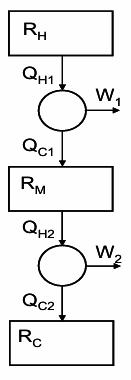
\includegraphics[width=0.14\textwidth]{images/3R-exemploentropia.png}
  \caption{Ilustração do Ciclo}
\end{wrapfigure}

Considerando três reservatórios de energia $R_H$, $R_M$ e $R_C$, e dois ciclos internamente reversíveis a operar entre estes: o primeiro ciclo opera entre os reservatórios $R_H$ e $R_M$, e o segundo entre os reservatórios $R_M$ e $R_C$. 

Os reservatórios, de volume constante, só trocam energia com as unidades de produção de trabalho dos ciclos e contêm a mesma massa do mesmo fluido incompressível com calor específico constante $c$.

Os reservatórios encontram-se inicialmente a $T_H$, $T_M$ e $T_C$, respetivamente. O sistema produz trabalho até os três reservatórios atingirem o equilíbrio térmico, onde as temperaturas dos reservatórios são igual a $T_f$.

\begin{eqnarray*}
    \Delta S = 0 \\
    \Delta S_H + \cancelto{0}{\Delta S_{ciclo_1}} + \Delta S_M + \cancelto{0}{\Delta S_{ciclo_2}} + \Delta S_C = 0 \\
    m c \ln \frac{T_f}{T_H} + m c \ln \frac{T_f}{T_M} + m c \ln \frac{T_f}{T_C} = 0 \\
    \ln \frac{T_f^3}{T_H T_M T_C} = 0 \\
    T_f = \sqrt[3]{T_H T_M T_C}
\end{eqnarray*}

Dado que o sistema produz trabalho, necessariamente: $T_H > T_M > T_C$, pelo que $T_C < T_f < T_H$, o que é um resultado correto: $T_H$ vai diminuindo fruto do calor cedido por $R_H$ ao ciclo, e $T_C$ vai aumentando e, portanto, a temperatura final terá de estar entres as duas temperaturas. 

O balanço de energia de todo o sistema dá:

\begin{eqnarray*}
    \Delta U = - W_1 - W_2 \\
    3 m c T_f - mc (T_H + T_M + T_C) = - W_T \\
    W_T =  mc \left[ (T_H + T_M + T_C) - 3 \sqrt[3]{T_H T_M T_C} \right] \\
\end{eqnarray*}

No entanto, se considerássemos que haveria irreversibilidades no sistema, obteríamos:

\begin{eqnarray*}
    \Delta S = \int \cancelto{0}{\frac{\delta Q}{T}} + \sigma \\
    m c \ln \frac{T_f^3}{T_H T_M T_C} = \sigma \\
    T_f = \sqrt[3]{T_H T_M T_C e^{\frac{\sigma}{m c}}}
\end{eqnarray*}

Assim, se $\sigma > 0$, $T_f \uparrow \implies W_T \downarrow$, e para $\sigma = 0$, obtemos $T_f = \sqrt[3]{T_H T_M T_C}$ ótimo, onde o trabalho total do sistema é máximo.

\end{examplebox}


\section{Trabalho em Sistemas Abertos}

O trabalho de um compressor ou uma turbina pode ser determinado da seguinte forma.

O balanço de energia, desprezando termos cinéticos e potenciais, dá:

\begin{eqnarray}
    \cancelto{0}{\frac{dE}{dt}} = \dot{Q} + \dot{W} + \dot{m} (h_1 - h_2) \\
    \frac{\dot{W}}{\dot{m}} = - \frac{\dot{Q}}{\dot{m}} + h_2 - h_1
\end{eqnarray}

O balanço de entropia dá, considerando a temperatura na fronteira do sistema constante:

\begin{eqnarray}
    \cancelto{0}{\frac{dS}{dt}} = \int \frac{\dot{q}}{T} + \dot{m} (s_1 - s_2) + \cancelto{0}{\dot{\sigma}}\\
    \frac{\dot{Q}}{T} = \dot{m} (s_2 - s_1) \\
    \frac{\dot{Q}}{\dot{m}} = T (s_2 - s_1)
\end{eqnarray}

De um modo geral, a temperatura pode variar, pelo que a expressão mais geral é:

\begin{equation}
    \left( \frac{\dot{Q}}{\dot{m}} \right)_{\substack{\text{int} \\ \text{rev}}} = \int_1^2 T ds
\end{equation}

onde o subscrito lembra-nos que a expressão é válida apenas para processos internamente reversíveis ($\sigma = 0$).

Assim, 
\begin{equation*}
    \frac{\dot{W}}{\dot{m}} = - \int_1^2 T ds + h_2 - h_1
\end{equation*}

De \ref{eq:2tds} ($ Tds = dh - v dp$), temos $-Tds + dh = v dp$, como $T=\text{const.}$, $\int -Tds + \int dh = \int v dp \Longleftrightarrow - \int T ds + \Delta h = \int v dp$.

Assim, obtemos o que pretendíamos

\begin{equation} \label{eq:w-intrev}
    \left( \frac{\dot{W}}{\dot{m}} \right)_{\substack{\text{int} \\ \text{rev}}} = \int_1^2 v dp
\end{equation}

onde o subscrito ``int. rev.'', indica que se refere ao trabalho total específico para um compressor/turbina internamente reversível. Localmente, pode-se dizer que as várias contribuições de trabalho $\delta W = - p dv$ resultam num trabalho global dado por esta expressão.

É de notar que a água, assim como outros líquidos considerados incompressíveis, com volume específico da ordem de grandeza $10^{-3}~\text{m}^3/\text{kg}$, aproximadamente constante, é muito mais fácil de comprimir, i.e. requer menos trabalho, do que um gás.
Considerando o ar gás ideal à temperatura e pressão ambiente, tem volume específico $v = \frac{RT}{p} = \frac{287 \cdot 298.15}{1\cdot 10^5} = 0.86~\text{m}^3/\text{kg}$, resultando num trabalho de compressão maior para a mesma pressão final.
Para o hidrogénio, $v = \frac{4124 \cdot 298.15}{1\cdot 10^5} = 12.3~\text{m}^3/\text{kg}$.

Assim, o trabalho específico para comprimir um kilograma de hidrogénio é muito maior do que um kilograma de água (1 kg de água ocupa $1~\text{L}$, enquanto 1 kg de hidrogénio $12000~\text{L}$). Quanto maior volume específico, maior o trabalho necessário para comprimir uma dada substância.

\subsection{Trabalho em Processos Politrópicos}

Para um processo politrópico $p v^n = c \implies v = \left(\frac{c}{p} \right)^{1/n}$:

\begin{itemize}
    \item Para $n \neq 1$:
    \begin{equation}
        \begin{split}
            \left( \frac{\dot{W}}{\dot{m}} \right)_{\substack{\text{int} \\ \text{rev}}} & = \int_{p_1}^{p_2} \left(\frac{c}{p} \right)^{1/n} \, dp  = c^{1/n} \frac{n}{n-1} \left(p_2^{1-1/n} - p_1^{1-1/n}\right)\\
            \left( \frac{\dot{W}}{\dot{m}} \right)_{\substack{\text{int} \\ \text{rev}}} & = \frac{n}{n-1} \left(p_2 v_2 - p_1 v_1\right), \quad n \neq 1
        \end{split}
    \end{equation}
    Para gás ideal:
    \begin{equation}
        \left( \frac{\dot{W}}{\dot{m}} \right)_{\substack{\text{int} \\ \text{rev}}} = \frac{n R}{n-1} \left(T_2 - T_1\right), \quad n \neq 1
    \end{equation}

    \item Para $n = 1$:
    \begin{equation}
        \begin{split}
            \left( \frac{\dot{W}}{\dot{m}} \right)_{\substack{\text{int} \\ \text{rev}}} & = \int_{p_1}^{p_2} \frac{c}{p} \, dp = c \ln \frac{p_2}{p_1}\\
            \left( \frac{\dot{W}}{\dot{m}} \right)_{\substack{\text{int} \\ \text{rev}}} & = p_1 v_1 \ln \frac{p_2}{p_1} = p_2 v_2 \ln \frac{p_2}{p_1}, \quad n = 1
        \end{split}
    \end{equation}
    Para gás ideal:
    \begin{equation}
        \left( \frac{\dot{W}}{\dot{m}} \right)_{\substack{\text{int} \\ \text{rev}}} = RT \ln \frac{p_2}{p_1}, \quad n = 1
    \end{equation}
\end{itemize}